\section{Dynamika}

\textbf{Zpětná vazba} (ZV) = proces, díky kterému se změna výstupních parametrů ($P$, $\Phi$) může podílet na změnu vstupních parametrů.\\

\textbf{Dynamika reaktoru} = to samé co kinetika, pouze už uvažuje zapojení ZV.\\

Cílem dynamiky reaktorů je řešit ZV. Vlivem ZV se nám totiž reaktivita mění (teplota, tlak, roztažnost...). Vše je primárně ovlivněno teplotou, jelikož s rosroucí reaktivitou roste výkon a tím i teplota systému. Celkovou reaktivitu můžeme určit jako součet reaktivity dodané zvenčí (tyče, palivo, konfigurace) a reaktivity ve ZV.\\

\subsection{Zpětné vazby}

ZV mohou být obecně:

\begin{itemize}
  \item kladné -- odezva roste, nestabilita.
  \item záporné -- odezva klesá, čímž se reaktor může stabilizovat,
\end{itemize}

Pokud se do reaktoru zavede kladná reaktivita s vlivem kladné zpětné vazby, a zároveň není-li reaktivita potlačena (tyčemi apod.), může i tato malá změna vést k nekontrolovanému nárůstu výkonu (rychlejší než exponenciální). Naopak, projeví-li se záporná zpětná vazba, reaktor se po chvíli stabilizuje. A na jaké hodnotě? Tehdy, pokud se reaktivity vyrovnají (kladná vnesená reaktivita se vyrovná záporné reaktivitě vziklé vlivem ZV $\rightarrow$ Celkový efekt je na nule), což závisí na velikosti vnesené reaktivity a velikosti zpětnovazebních koeficientů. Záporné ZV pomáhají k řízení reaktoru, jelikož vždy působí proti počáteční změně a mají tendenci reaktor stabilizovat, viz graf \ref{ZV}.

\begin{figure}[H]
  \centering
  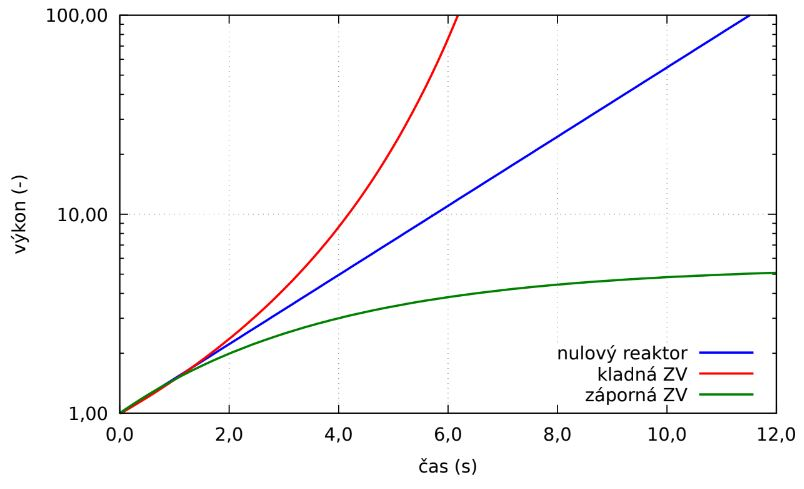
\includegraphics[width=0.7\textwidth]{img/ZV.JPG}
  \caption{Vliv ZV na zavedení kladné reaktivity.}
  \label{ZV}
\end{figure}

Graf dále ukazuje, že při velmi nízkých výkonech (nulový reaktor) všechny křivky splývají, jelikož se vliv ZV zatím neuplatňuje. Lze tedy říci, že každý reaktor se chová jako nulový a každý reaktor má ZV, pouze závisí, od jakého výkonu se začnou projevovat.\\

Dále je možné ZV rozlišit pomocí fyzikálních vlastností:

\begin{itemize}
  \item jaderné -- změnou teploty se mění mikroskopické účinné průřezy (Doppler), zároveň se může změnit Maxwell-Boltzmannovo rozdělení hustoty toku (maximum se posune do vyšších energií), což má za následek změnu reakčních rychlostí,
  \item hustotní -- změnou teploty se mění hustota jader a tím makroskopické účinné průřezy, nebo geometrické změny ovlivní Buckling.
\end{itemize}

\subsubsection{Doppler}

Dopplerovo rozšíření je kapitola sama o sobě. To se uplatňuje pouze v rezonancích, kde vlivem teplotní změny dochází k poklesu maxima a nárůstu šířky peaku tak, aby plocha pod peakem zůstala konstantní (vlivem teplotní změny atomy více kmitají, a proto se jakoby "rozmazávají"). Jelikož neutron ztrácí svoji energii po skocích, ne kontinuálně, při rozšíření základny rezonance vzniká "větší prostor", kam může neutron spadnout a dojít k záchytu.\\

Ve výsledku, Dopplerovo rozšíření vždy způsobuje zvyšování abrosbce, otázka je, jestli jde o radiační záchyt, nebo štěpení. Pro okolní materiály mimo palivo (moderátor, chladivo, konstrukce) vždy dochází k radiačnímu záchytu, jde tedy o zápornou ZV která vede k poklesu reaktivity.\\

U paliva záleží na konkrétním izotopickém složení a obohacení. Například pro U-238 je Doppler velmi významný, jelikož při zpomalování neutronu už ho neutron nemůže štěpit a dochází právě k radičnímu záchytu. Naopak u U-235 by sice došlo k nárůstu absorbce, ale tím i nárůstu štěpení. Je proto důležitý poměr obohacení. Na KIDu jsme si říkali, že při obohacení pod 35\% dojde vždy k převládnutí parazitní abrosrbce na U-238 a tedy k poklesu reaktivity. Pod touto hranicí jde tedy o zápornou ZV (tepelné reaktory), nad tuto hranici je třeba být opatrný, jelikož může vést ke kladné ZV (rychlé reaktory).

\subsubsection{Vodo-uranový poměr}

Tepelné jaderné reaktory potřebují k udržení štěpné řetězové reakce tepelné neutrony, které vznikají zpomalováním v moderátoru. Při změně teploty moderátoru dochází rovněž ke změně jeho hustoty a tím i ke změně makroskopických průřezů a reakčních rychlostí. Při změně teploty moderátoru tak nutně dochází ke změně moderačních vlastností a tím i ke změně reaktivity.\\

Aby bylo možné analyzovat, jak se změna hustoty moderátoru projeví na změně reaktivity, je třeba určit průběh závislosti reaktivity na hustotě moderátoru (\textbf{vodo-uranový poměr}), viz obrázek \ref{voda-uran}. Z toho lze rozlišit 2 typy moderátoru:

\begin{itemize}
  \item ideální moderátor (modrý) -- moderátor, na kterém nedochází k žádné parazitní absorbci,
  \item skutečný moderátor (červená).
\end{itemize}

\begin{figure}[H]
  \centering
  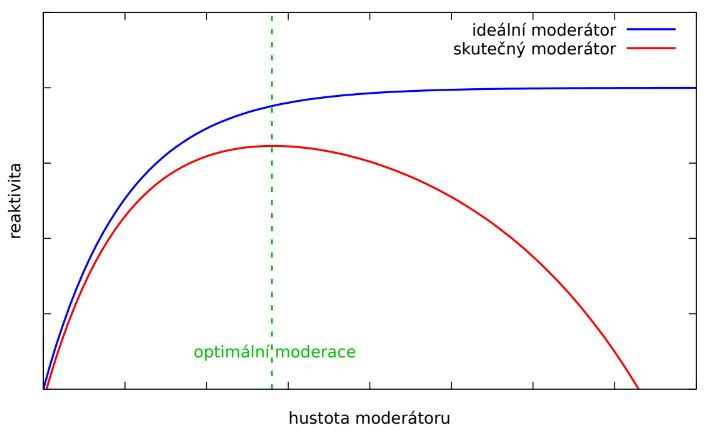
\includegraphics[width=0.7\textwidth]{img/voda-uran.JPG}
  \caption{Závislost reaktivity na hustotě moderátoru.}
  \label{voda-uran}
\end{figure}

Při přidávání ideálního moderátoru dochází pouze k větší termalizaci a žádné parazitní absorbci, proto reaktivita roste a ustaluje se na saturované hodnotě. Ve skutečnosti ale při přidávání moderátoru od jistého okamžiku dojde k převládnutí parazitní absorbce a reaktivita opět klesá. K maximu reaktivity pak dochází při tzv. \textbf{optimální moderaci}, část vlevo se poté nazývá \textbf{podmoderovaná} (méně moderátoru než je optimum) a část vpravo \textbf{přemoderovaná}. Tvar této křivky závisí na konkrétním moderátoru (zde je vidět např. výhoda těžké vody oproti lehké vodě, kdy na těžké dochází k absorbci výrazně méně).\\

Známe-li tyto grafy, je možné analyzovat, co se stane při změně teploty. Při zvyšování teploty dojde k poklesu hustoty moderátoru, což v řeči grafu \ref{voda-uran} znamená posun doleva. Pokud se budeme nacházet v podmoderované oblasti, dojde k poklesu reaktivity (ZV). Nicméně v přemoderované oblasti dojde k nárůstu (kladná ZV). Z hlediska bezpečnosti je proto důležité mít reaktor v podmoderované oblasti, což je možné ovlivnit: geometrií, obohacením, vyhořením, koncentrací boru apod. Zároveň může docházet k lokálnímu přemoderování (výzkumné reaktory), důležité je ale celkový charakter.

\subsection{Zpětnovazební koeficienty reaktivity}

\textbf{Zpětnovazební koeficienty} mohou být jakékoliv (teplotní, hustotní, výkonové), nicméně většinou je stejně vše ovlivněno právě teplotou (teplota ovlivní hustotu, změna výkonu ovlivní teplotu apod.), tudíž se dále zaměříme pouze na ty teplotní. Ty je možné určit dle vztahu:

\begin{equation}
  \boxed{
  a_i = \dfrac{\partial \rho}{\partial T_i}
  \label{zpetnovazebni_koeficient_definice}
  }
\end{equation}

A celkový vliv na reaktivitu jako:

\begin{equation}
  \boxed{
  \rho_{tot} = \sum_i \dfrac{1}{V_i} \int_{V_i} a_i(\bar{r}) \Delta T_i(\bar{r}) \Omega_i(\bar{r}) d\bar{r},
  \label{zpetnovazebni_koeficient_reaktivita}
  }
\end{equation}

kde:

\begin{itemize}
  \item $\Delta T_i$ -- představuje teplotní odchylku od i-té složky (teplotní rozdíl od kritického a aktuálního stavu),
  \item $\Omega_i$ představuje tzv. \textbf{normovanou váhovou funkci}, která opravuje fakt, že stejné teplotní změny mohou mít v jiných místech jiný vliv na reaktivitu. Skutečně jsou úměrné $\Phi^2$.
\end{itemize}

Při použití jednobodové kinetiky je možné zanedbat prostorovou závislost. Pokud se navíc zavede lineární model zpětné vazby, kdy budou koeficienty konstantní (normálně jsou závislé na teplotě), tak se výpočet zjednodušší:

\begin{equation}
  \boxed{
  \rho_{tot} = \sum_i a_i \Delta T_i (t).
  \label{zpetnovazebni_koeficient_reaktivita_1B}
  }
\end{equation}

\subsection{Přenosová funkce zpětné vazby}

Vliv zpětně vazby je možné vyjádřit i pomocí jednobodové kinetiky/dynamiky. Z linearizovaného modelu nulového reaktoru vyplývá (směr "doprava", tedy jak změna reaktivity vede na změnu četnosti):

$$ \dfrac{\Delta \tilde{N}(s)}{N_0} = \tilde{G_0}(s) \cdot \tilde{\rho}(s) = \tilde{G_0}(s) \cdot [ \tilde{\rho_\text{ex}}(s) + \tilde{\rho_\text{ZV}}(s) ], $$

kde $\tilde{\rho_\text{ex}}(s)$ značí vnesenou reaktivitu a $\tilde{\rho_\text{ZV}}(s)$ reaktivitu zpětné vazby. Zároveň je ale tato ZV reaktivita ovlivněna změnou četnosti, proto musí mít vlastní \textbf{přenosovou funkci zpětné vazby} $\tilde{W_\text{ZV}}(s)$, pro kterou platí\footnote{Tentokrát se přenosová funkce ZV definuje "obráceně", viz linearizovaný model v předešlé otázce. Tudíž pro $G_0$ platí, že změna reaktivity ovlivní četnost, ale tady platí, že změna četnosti ovlivní velikost ZV reaktivity.} (směr "doleva", tedy jak změna četnosti ovlivní reaktivitu, nicméně tentokrát pouze tu zpětnovazební):

$$ \tilde{\rho_\text{ZV}}(s) = \tilde{W_\text{ZV}}(s) \cdot \dfrac{\Delta \tilde{N}(s)}{N_0}. $$

Když se to všechno poskládá do sebe, tak je možné získat finální tvar spolu s tzv. \textbf{přenosovou funkcí reaktoru}\footnote{Tentokrát už nenulového.} $\tilde{G}(s)$ ve tvaru:

\begin{equation}
  \boxed{
    \dfrac{\Delta \tilde{N}(s)}{N_0} = \tilde{G}(s) \cdot \tilde{\rho}(s) = \dfrac{\tilde{G_0}(s)}{1 - \tilde{G_0}(s) \tilde{W_\text{ZV}}(s)} \cdot \tilde{\rho}(s).
  }
\end{equation}

Zbývá určit pouze tvar přenosové funkce zpětné vazby, čímž se získá tvar celkové přenosové funkce a vše se může řešit stejnými postupy, jako v případě kinetiky.\\

Zároveň se ještě hodí znát podmínku stability reaktoru, tedy situaci, jestli se výkon po nějaké době ustálí, nebo diferguje do nekonečna. Zde platí jednoduchý vztah:

\begin{equation}
  \boxed{
    \int_0^\infty  |G(t)| dt < \infty.
  }
\end{equation}

Zde platí, že nulový reaktor je vždy nestabilní. Stabilizuje se pouze až se zápornými ZV.

\subsection{Modely dynamiky reaktoru}

Analytické vyjádření zpětnovazební přenosové funkce je obtížné, často se musí něco zanedbat apod. Existuje několik modelů v závislosti na tom, co se mění (ve všech případech jde o linearizované modely):

\begin{itemize}
  \item Dvousložkový model -- mění se pouze teplota paliva a chladiva (tlakovodní a sodíkové reaktory):\\
  $$ \tilde{W_\text{ZV}}(s) = \dfrac{a_\text{fuel} (1 + s \: \tau_\text{cool}) + a_\text{cool} \: \Gamma}{k_\text{fuel} \: [(1 + s \: \tau_\text{cool})(1 + s \: \tau_\text{fuel}) - \Gamma]} $$
  \item Jednosložkový model -- pouze jedna teplota (molten salt):\\
  $$ \tilde{W_\text{ZV}}(s) = \dfrac{a_\text{power}}{1 + s \: \tau}. $$
  \item Adiabatický model -- rychlé změny, kdy se teplo nestačí odvézt:\\
  $$ \tilde{W_\text{ZV}}(s) = \dfrac{a_\text{fuel}}{s \: C_\text{fuel}}. $$
\end{itemize}

Ve všech případech: $a$ značí koeficient reaktivity, $C$ tepelnou kapacitu, $k$ součinitel prostupu tepla a konstanty $\tau$ a $\Gamma$ jsou jisté časové, resp. bezrozměrné konstanty, které pouze zjednodušují zápis a pro každý model se volí jinak. Více modelů a jejich odvození je v Bédových skriptech.

